\chapter{矩阵乘优化与性能评估}\label{chap:GEMMOpt}

\section{实验配置}

本文实验的测试环境包括AMD Fiji服务器和AMD Vega服务器,其中每个服务器都是单节点,所用ROCm平台和操作系统版本相同。每个计算节点的软硬件主要参数如表\ref{tab:hardwareplatform}所示。
\begin{table}[htbp]
	\bicaption{实验平台软硬件主要参数}{Experimental platform hardware main parameters}
	\label{tab:hardwareplatform}
	\begin{center}
		\begin{tabular}{ | l | p{6cm} | p{6cm} |}
			\hline
			服务器 & AMD Fiji服务器 & AMD Vega服务器 \\ \hline
			GPU & Fiji R9 Nano & 2 x Vega10 \\ \hline
			%CPU & Intel(R) Xeon(R) CPU E5-2680 v3 @ 2.50GHz & 2 AMD EPYC 7451 24-Core Processor \\ \hline
			内存 & 251GB DDRM & 251GB DDRM \\ \hline
			操作系统 & Ubuntu16.04 & Ubuntu16.04 \\ \hline
			操作系统内核 & rocm-1.7 & rocm-1.7 \\ \hline
			OpenCL C version & OpenCL C 2.0 & OpenCL C 2.0 \\ \hline
			PCIe version & PCIe Gen3 & PCIe Gen3 \\
			\hline
		\end{tabular}
	\end{center}	
\end{table}


\section{矩阵乘性能调优}

\subsection{寄存器分块对v\_mac指令占比的影响}
\begin{figure}[htbp]
	\centering
	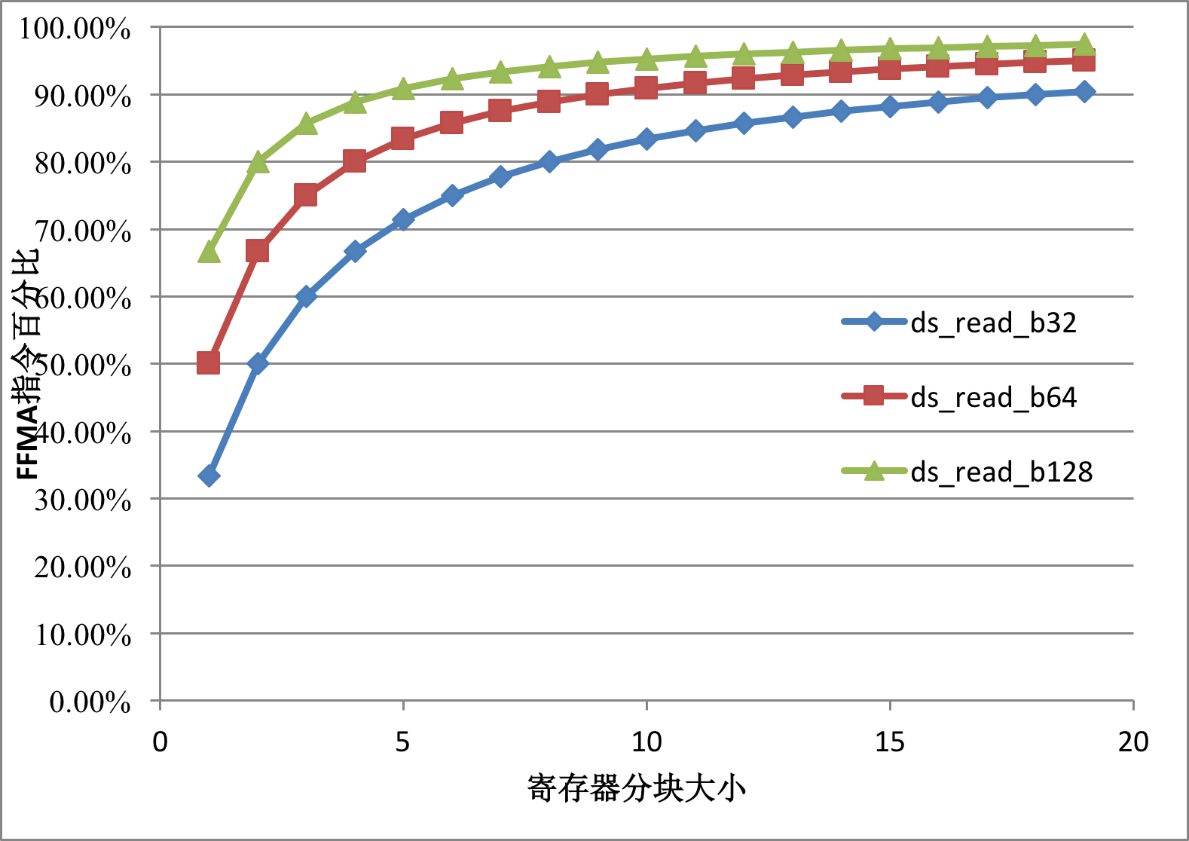
\includegraphics[width=0.60\textwidth]{ffma_percentage}
	\bicaption{v\_mac指令百分比随着寄存器分块大小的变化趋势}{The percentage of v\_mac instruction changes with the size of the register block}
	\label{fig:ffma_percentage}
\end{figure}

从上图\ref{fig:ffma_percentage}中可以看出,随着寄存器分块大小增大,v\_mac指令百分比在提高。在寄存器分块大小不变的情况下,ds\_read\_bxx指令的位数宽度越宽,v\_mac指令百分比越高。如果采用的寄存器分块大小为6,则FFMA/DS\_READ\_B32=4:1,FFMA/DS\_READ\_B64=8:1,FFMA/DS\_READ\_B128=16:1。FFMA指令的百分比分别为80\%,88.89\%和94.12\%。

增大寄存器分块可以提高v\_mac指令的百分比,在v\_mac和ds\_read混合指令通量不变的情况下,v\_mac指令的百分比越高,v\_mac指令的通量越高。

\subsubsection{使用更宽的数据读指令}
为了实现更好的性能,在编写矩阵乘程序时,十分有必要将辅助指令的占比减到最小。这里的辅助指令是指非计算指令,尤其是指ds\_read指令。AMD GPU汇编提供了ds\_read\_b32,ds\_read\_b64和ds\_read\_b128指令,分别可从shared memory一次读32bit,64bit和128bit数据。使用更宽的读数据(load)指令可以减少ds\_read指令的数量。

对于AMD Fiji和Vega GPU,每个CU每一个shader cycle的ds\_read指令通量的峰值为32个32-bit。AMD GPU每个CU上每个SIMD有16个LD/ST单元,使用ds\_read\_b64就可以满足通量峰值,所以使用ds\_read\_b128指令不会增加读数据的通量。此时,在ds\_read\_b64和ds\_read\_b128和v\_mac混合指令通量相同的情况下,最好的情况是合理使用ds\_read\_b128指令,使用ds\_read\_b64的通量峰值将是ds\_read\_b32通量峰值的2倍。


\subsection{workgroup大小对访存带宽的影响}
根据workgroup的大小可以计算出所需的全局访存量,一个workgroup的计算任务为$b_m \times b_n$,$A$矩阵的维度为$M \times K$,$B$矩阵的维度为$K \times N$,由此可以计算出全局访存量为
\begin{equation}
\label{eq:globalmem}
\frac{M}{b_m} \times \frac{N}{b_n} \times K \times (b_m + b_n) = M \times N \times K \times (\frac{1}{b_m} + \frac{1}{b_n})
\end{equation}

由公式\ref{eq:globalmem}可知一个workgroup的计算量越多,全局访存量越少,但随着一个workgroup计算量的增多,其所需的局部共享内存也会增多,由于局部共享内存是一个CU上的有限资源,因此一个CU上并发的workgroup数会减少。对GPU而言CU上并发的workgroup数越多,越能隐藏高访存延迟。综上所述,workgroup大小会同时影响全局访存量和访存延迟隐藏。

\begin{table}[htbp]
	\bicaption{一个线程的数据搬移方向和搬移量}{Data movement direction and volume of a thread}
	\label{tab:thread_data_move}
	\begin{center}
		\begin{tabular}{ | l | l | }
			\hline
			Data path & Volume  \\ \hline
			global $\Rightarrow$ register & $\frac{r_x \times r_y}{b_n} \times b_k + \frac{r_x \times r_y}{b_m} \times b_k$  \\ \hline
			register $\Rightarrow$ shared & $\frac{r_x \times r_y}{b_n} \times b_k + \frac{r_x \times r_y}{b_m} \times b_k$  \\ \hline
			shared $\Rightarrow$ register & $r_x \times b_k + r_y \times b_k$ \\
			\hline
		\end{tabular}
	\end{center}	
\end{table}
在最内层循环中,每个线程共$2 \times r_x \times r_y$个浮点操作。表\ref{tab:thread_data_move}列出了主循环过程中一个线程的数据搬移方向和搬移量,包括全局内存到寄存器、寄存器到局部共享内存和局部共享内存再到寄存器。这样做的目的是充分挖局部共享内存和寄存器的数据重用。我们定义局部共享内存的计算密集度(Load data share arithmetic intensity)为浮点操作次数与局部共享内存访存次数的比例,其公式可表达如下\ref{eq:shared_arith_intensity}
\begin{equation}
\label{eq:shared_arith_intensity}
ldsAI = \frac{2 \times r_x \times r_y \times b_k}{r_x \times b_k + r_y \times b_k} = \frac{2}{\frac{1}{r_x} + \frac{1}{r_y}}
\end{equation}

每个线程需要$r_x$、$r_y$和$r_x \times r_y$分别存储A矩阵的一子列、B矩阵的一子行和C子矩阵。为了隐藏局部共享内存的访存延迟,我们使用了寄存器双缓冲。因此需要额外的$r_x$和$r_y$来预取下一次循环的A和B。由于所有寄存器总数不超过256的限制,我们可以得到公式\ref{eq:register_limit}
\begin{equation}
\label{eq:register_limit}
2 \times r_x + 2 \times r_y + r_x \times r_y < 256
\end{equation}
从公式\ref{eq:shared_arith_intensity}可知,寄存器分块越大局部共享内存计算密集度越高,在公式\ref{eq:register_limit}的限制条件下,当$r_x = r_y$时公式\ref{eq:shared_arith_intensity}取到最优值。因此寄存器分块可以选择$4\times 4$、$6\times 6$、$8\times8$、$12\times 12$等。
\section{汇编层次调优}
实际的SGEMM性能不会超过预估的SGEMM性能上界。对性能上界的评估比较理想化,因为这里主要考虑了影响性能的几个主要因素。除了前面考虑到的几个因素,也有其他因素可能会影响性能。实际的性能上界将介于预估性能上界和实际SGEMM性能之间。

根据A,B矩阵是否转置,可将SGEMM kernel可分4种情况,NN,NT,TN,TT(N表示不转置,T表示转置)。这里的分析中,主要考虑了两种类型的指令v\_mac和ds\_read\_bxx。在SGEMM中,还有其他的“辅助”指令对GFLOPS并没有贡献。“辅助”指令包括全局内存地址计算指令,shared memory地址计算指令等。同时,也没有考虑barrier指令对性能的影响。但实际上任何barrier指令都会降低程序性能。

\subsection{汇编调优的必要性}
使用高级语言(如OpenCL,CUDA)编写GPU程序的好处是开发速度快、易维护,但其对指令的控制能力相对较弱,同时程序编制人员对编译器的具体行为无法预测。有时编程人员对OpenCL或CUDA kernel所进行的手工优化可能会被编译器忽略掉,所以有时候编程人员编写的GPU程序性能会取决于编译器是否友好。

通过编写汇编kernel,编程人员可以直接跳过编译器,面向GPU硬件指令编程。这使得编程人员有机会进行更细粒度的程序调优。可以通过数据预取、寄存器双缓冲、shared memory双缓冲、bank冲突消除、指令重排等手法进行矩阵乘调优。其中OpenCL和汇编都可以使用数据预取,寄存器双缓冲和shared memory双缓冲和bank冲突消除这些手法进行程序优化。但只有通过汇编,程序编制人员才能进行细粒度的指令重排。在大量乘加指令之间的合适位置插入访存指令,尽可能用计算掩盖访存延迟,使得矩阵乘主循环中v\_mac指令通量接近v\_mac通量上界。

图\ref{fig:opencl_gemm_1_1_replot}展示了OpenCL实现的矩阵乘不同优化方法的性能比较。

\begin{figure}[htbp]
	\centering
	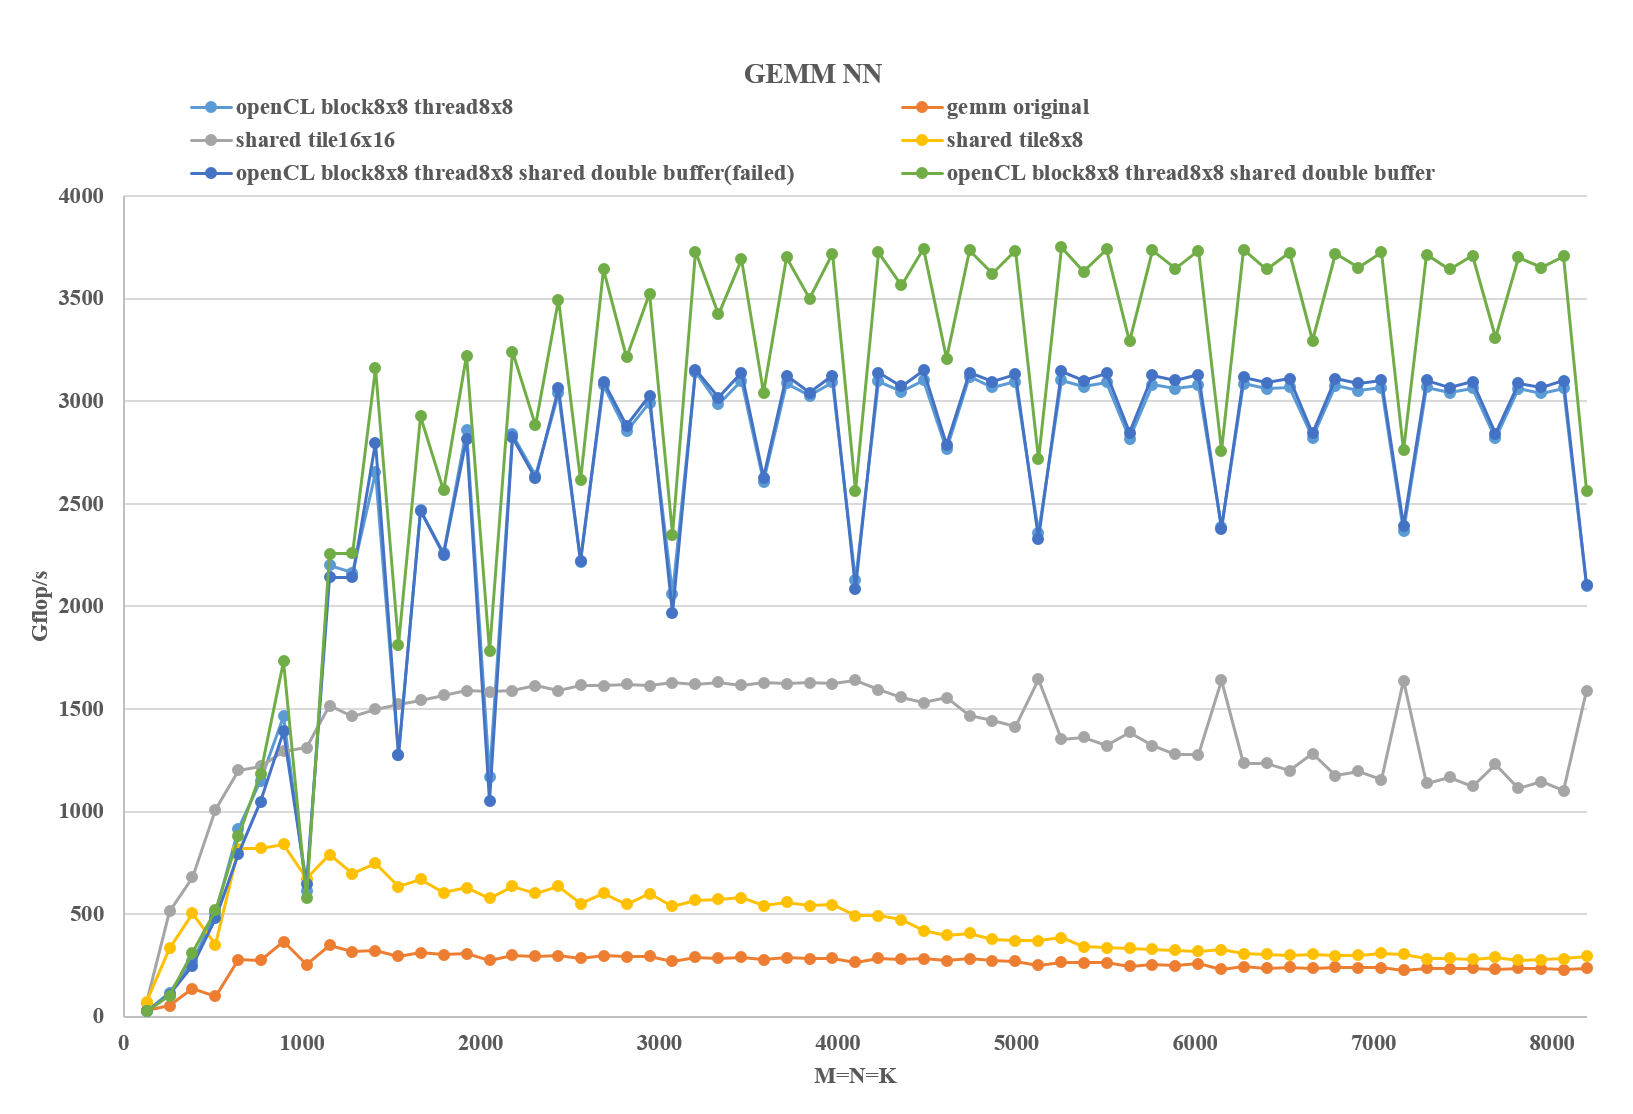
\includegraphics[width=0.80\textwidth]{opencl_gemm_1_1_replot}
	\bicaption{矩阵乘OpenCL实现性能比较}{Comparison of GEMM performance implemented by OpenCL}
	\label{fig:opencl_gemm_1_1_replot}
\end{figure}

从图\ref{fig:opencl_gemm_1_1_replot}可以看出,最简单的矩阵乘GPU实现其浮点效率最低(图\ref{fig:opencl_gemm_1_1_replot}中的gemm original曲线)。gemm original的实现没有使用shared memory,采用內积法每个线程计算一个输出。中间两条曲线表示使用shared memory,分块大小分别为8x8和16x16。由于矩阵乘在计算过程中有很多数据重用,利用数据重用的特点,将要计算的数据预先读入shared memory。在真正计算时从shared memory中取数据,可以减小数据读延迟。图\ref{fig:gemm_inner_product_tile}展示了使用shared memory分块的內积法矩阵乘。可以看出,计算C矩阵分块的同一行时,需要重复读A矩阵分块的同一行4个元素;同理,计算C矩阵分块的同一列时,要重复读B矩阵分块的同一列4个元素。全局内存读的次数减少4倍。分块大小为8时,全局内存读次数将减少8倍。所以在内存带宽受限时,提高shared memory分块大小可以减少全局内存读,降低内存带宽压力,提高计算性能。从图\ref{fig:opencl_gemm_1_1_replot}中可以看出16x16分块的性能高于8x8分块。

图\ref{fig:opencl_gemm_1_1_replot}中曲线openCL block8x8 thread8x8是原始的外积法矩阵乘实现。该矩阵乘的参数配置是,一个threadblock的线程数为8x8=64,在AMD GPU上即一个wavefront的大小。每个线程计算8x8的分块,因此一个threadblock计算64x64的输出。循环展开次数为8。写回结果时,直接从寄存器写回到全局内存。可见,外积法的矩阵乘性能从整体上要优于內积法。这是由于采用內积法可以并行地计算所有的乘法,但不能并行的计算加法。即使可以使用reduction来快速计算加法,但仍然会产生很多空闲的线程。这样,由于任务划分的不均衡,会使得计算性能大大降低。然而,如果用外积法来代替內积法,将会很大程度上缓解负载不均衡带来的性能损失。曲线openCL block8x8 thread8x8 shared double buffer表示在原始外积法实现的基础上进行了shared memory双缓冲的优化,性能得到进一步的提升。

\begin{figure}[htbp]
	\centering
	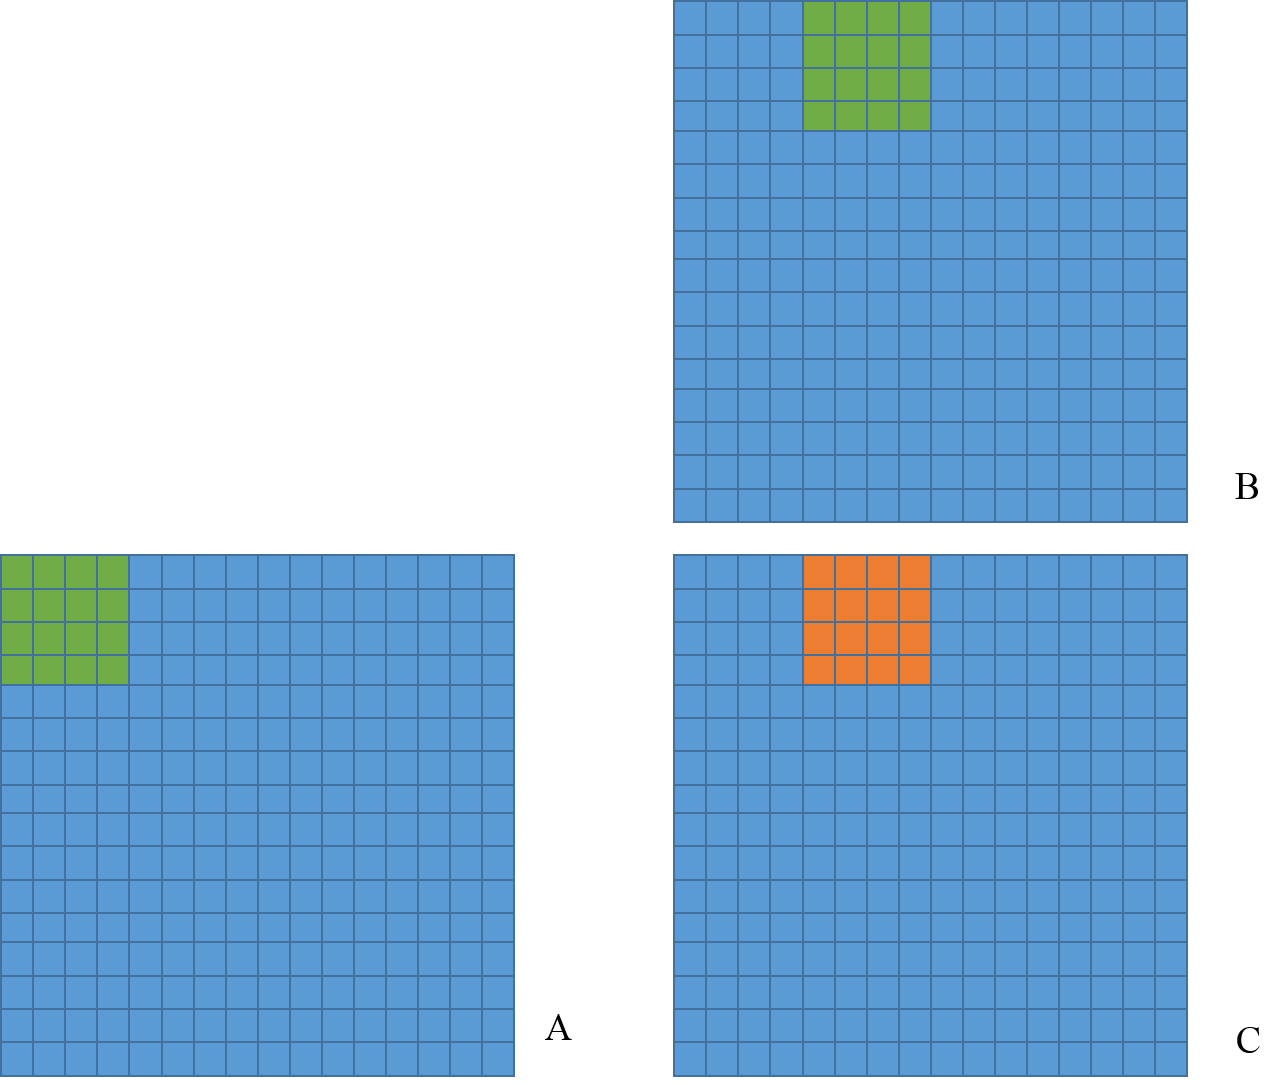
\includegraphics[width=0.60\textwidth]{gemm_inner_product_tile}
	\bicaption{內积法矩阵乘shared memory分块图示说明}{Illustration of inner-product GEMM with shared memory block}
	\label{fig:gemm_inner_product_tile}
\end{figure}

接下来进行外积法矩阵乘的shared memory bank冲突分析。图\ref{fig:shared_memory_bank_dist}展示了shared memory bank的分布情况。这里首先介绍一下AMD GPU shared memory的bank设计,shared memory有32的bank,每个bank的宽度为4字节。图\ref{fig:shared_memory_bank_dist}中绿色部分表示bank编号,蓝色部分表示一个block中A矩阵在shared memory中的分布情况,蓝色部分的同一列位于相同的bank。图中用其他颜色标注的部分,表示每个线程要读取的数据,例如(0,xxx)表示tid.x == 0,tid.y为0$\sim$7的线程要读取的8个元素。可以看出(0,xxx)线程和(4,xxx)线程都要读取bank0$\sim$bank7中的元素。图\ref{fig:bank0}展示了所有线程读bank0的情况。可以看出bank0的读取有4-way bank冲突。其他bank可类似分析。可以得知对于所有的bank,此时的shared memory有4-way bank冲突。

%bank冲突消除:


\begin{figure}[htbp]
	\centering
	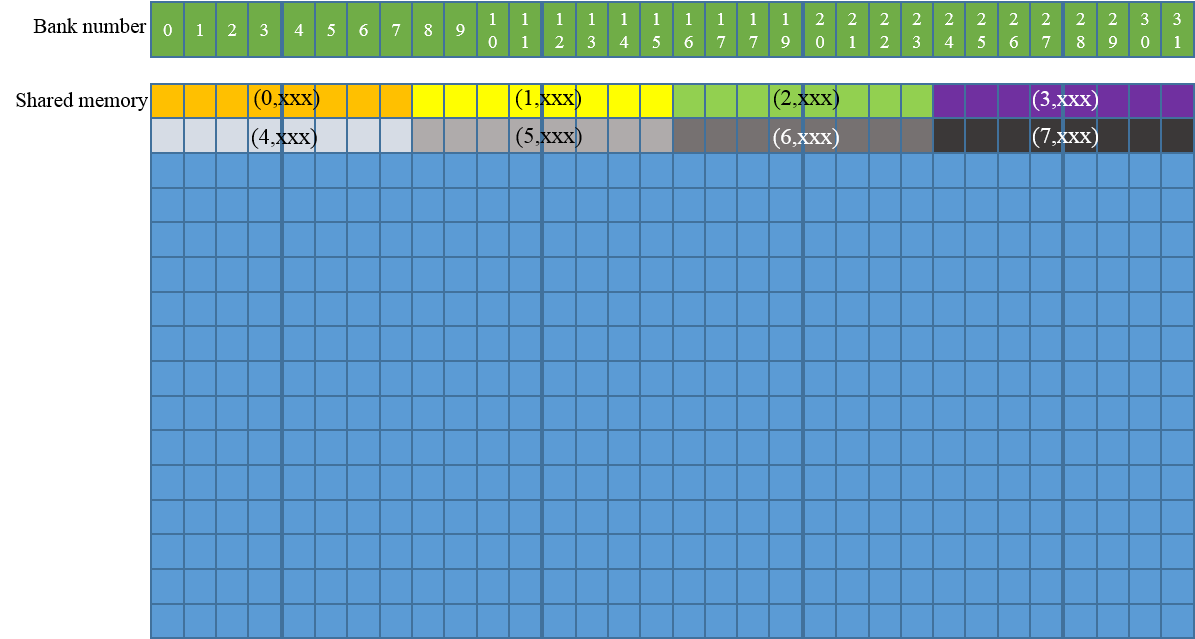
\includegraphics[width=0.80\textwidth]{shared_memory_bank_dist}
	\bicaption{shared memory bank分布}{Distribution of shared memory bank}
	\label{fig:shared_memory_bank_dist}
\end{figure}

\begin{figure}[htbp]
	\centering
	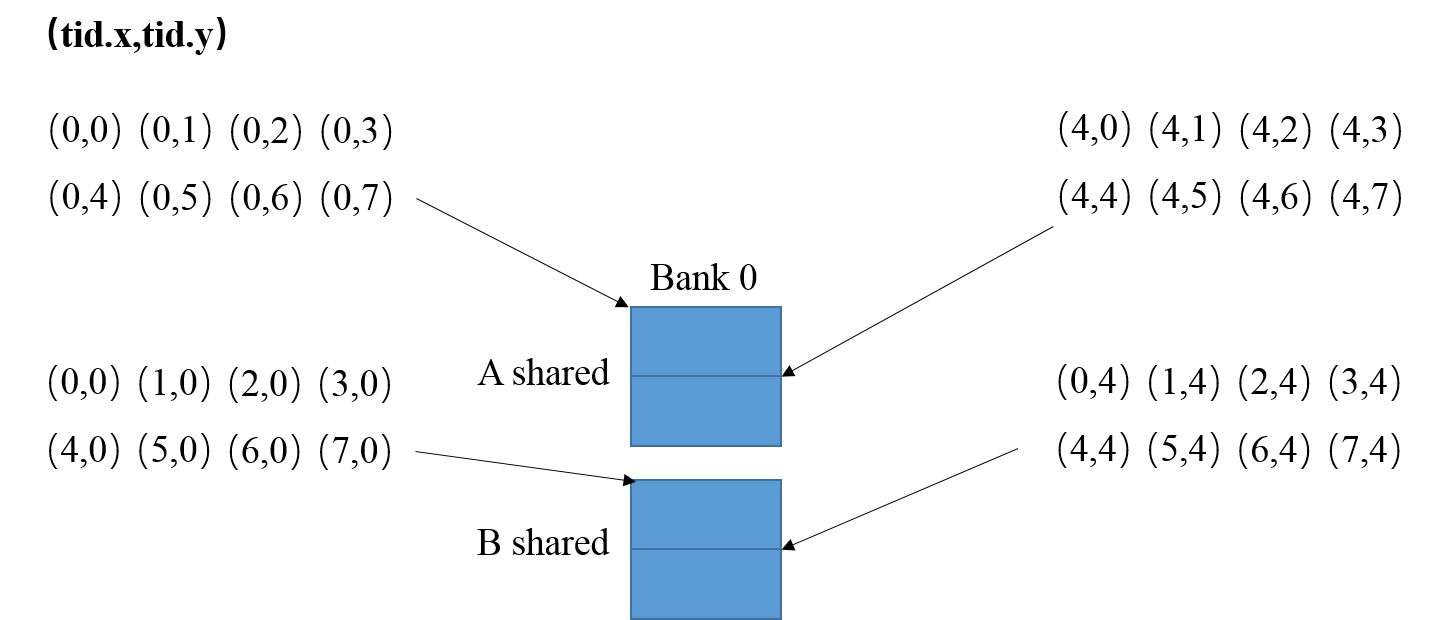
\includegraphics[width=0.80\textwidth]{bank0}
	\bicaption{4-way shared memory bank冲突}{4-way shared memory bank conflict}
	\label{fig:bank0}
\end{figure}

\subsection{优化内存访问}
汇编语言的访存优化和用高级语言(如CUDA,OpenCL)优化访存比较类似。一个wavefront(warp)中线程的全局访存请求可以合并成一到多个内存事务(memory transactions)。合并的方式和具体的GPU访存模式有关。为了高效的访问全局内存,通常我们安排一个wavefront中的线程访问全局内存中一段连续内存区域的数据。这样容易进行全局访存合并。在SGEMM程序的主循环中,主要的指令为v\_mac和ds\_read,为了提高v\_mac指令的百分比,减少ds\_read指令的数目就变得尤为关键。在前面的介绍中,讲到了可以通过使用DS\_READ\_B64或DS\_READ\_B128来减少DS\_READ指令数量。在shared memory中,线程读取A,B子矩阵也应该可以进行访存合并,我们安排每个线程可以读取连续的A,B子矩阵,一个wavefront中的线程可合并访问shared memory。同时,为了减少甚至消除shared memory的bank冲突和满足DS\_READ指令对齐的要求,在必要的时候,编程人员需要在shared memory中合理的进行填充。

\begin{figure}[htbp]
	\centering
	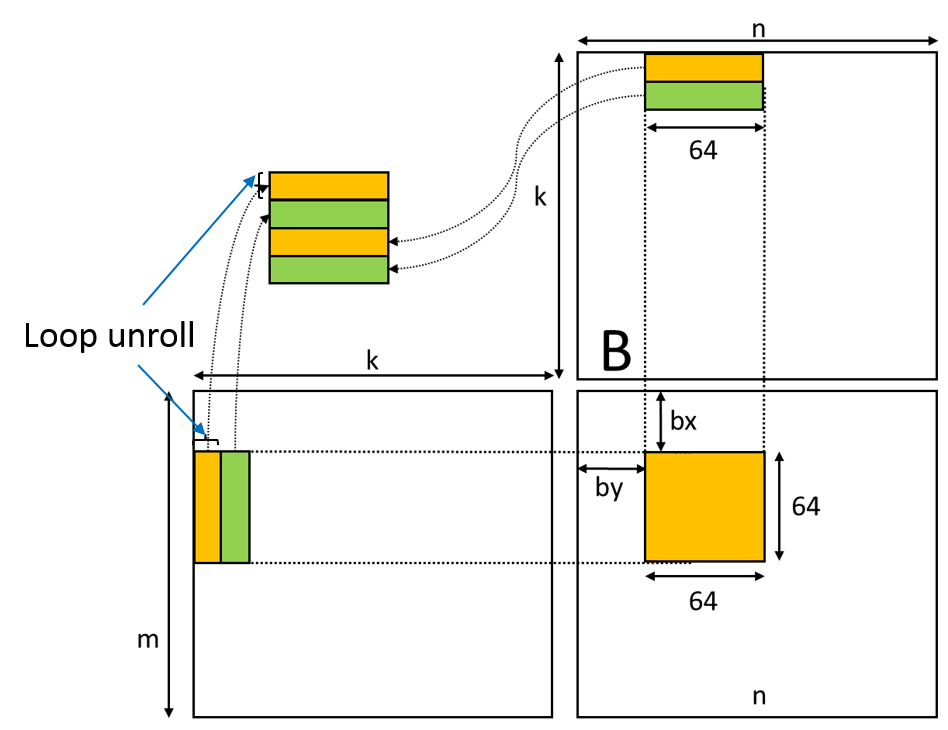
\includegraphics[width=0.50\textwidth]{loop_unroll_replot}
	\bicaption{循环展开图示}{Loop unroll}
	\label{fig:loop_unroll_replot}
\end{figure}
\subsection{循环展开}
通过循环展开(如图\ref{fig:loop_unroll_replot}),可以提高指令的通量。如下图中所示,沿着K方向做循环展开,这样在每次循环产生更多的浮点乘加操作,充分利用GPU上每个线程可拥有的寄存器个数。并且以循环展开作为前提,可以做后续的寄存器双缓冲,局部共享内存双缓冲等优化。通常都是做偶数次展开,这是为后面双缓冲要恰好是2的倍数做准备。在这里循环展开8次,考虑的因素有寄存器个数的限制,和局部共享内存容量的限制。循环展开的好处是能够减少很多冗余指令,减少分支判断指令的数目。对于GPU而言,执行分支判断指令只要用到标量部件就可以了,这极大浪费了GPU的向量计算单元,致使程序性能降低。

图\ref{fig:gemm_manual_unroll}展示了手工进行循环展开带来的性能提升。为了尽量避免OpenCL编译器的未知行为,编程人员可以进行手工循环展开。对于GPU而言,执行分支指令时大量的运算部件就处于空闲状态,这极大浪费了GPU大量的计算部件。手工循环展开的一个好处是可以减少分支指令的执行次数,给编程人员留出更多的优化空间。
\begin{figure}[htbp]
	\centering
	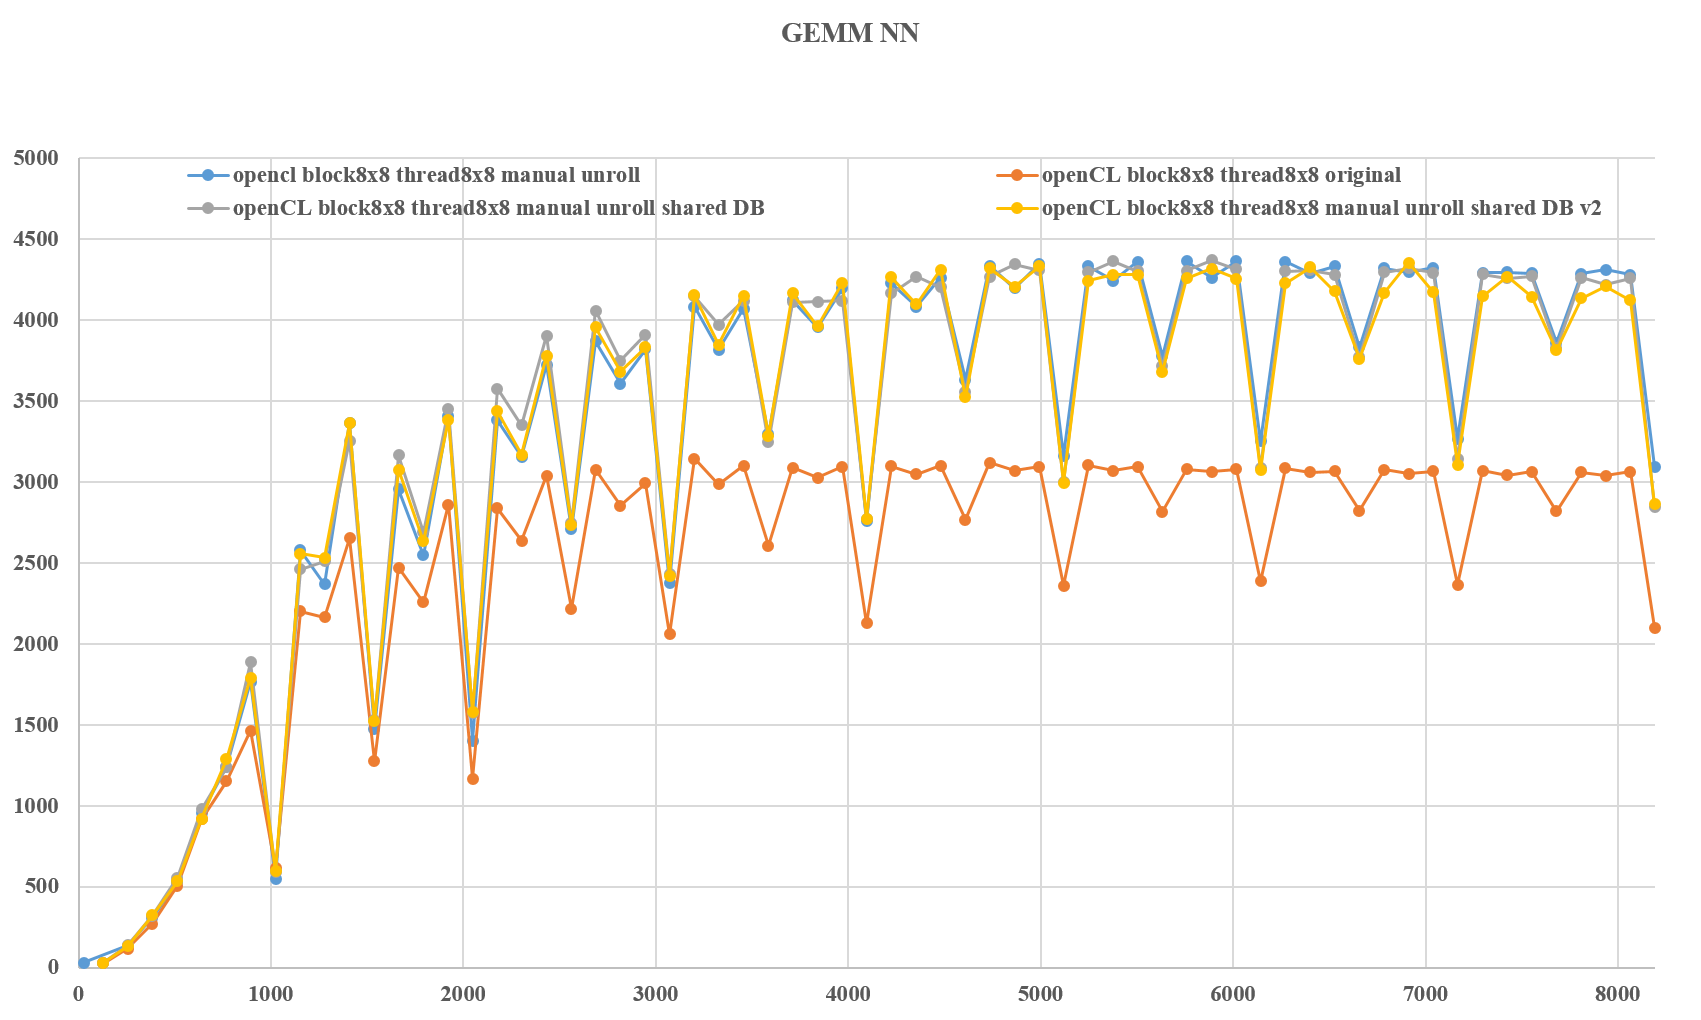
\includegraphics[width=0.80\textwidth]{gemm_manual_unroll}
	\bicaption{手工循环展开带来的性能提升}{Manual loop unroll}
	\label{fig:gemm_manual_unroll}
\end{figure}
\subsection{数据预取}
通过数据的预取可以减小计算时读取数据产生的等待延迟。从全局内存预取数据到共享内存,以增加一倍局部共享内存的代价来掩盖全局内存的访存延迟;从局部共享内存预取数据到寄存器,以增加一倍寄存器的代价来掩盖局部共享内存访存的延迟。

\subsection{shared memory双缓冲}
在前面的矩阵乘GPU算法描述中,讲述了shared memory的使用方法。首先将数据从全局内存读入寄存器,然后从寄存器写回到shared memory,最后再从shared memory读取数据到寄存器,并在寄存器中做计算。

为了更有效地利用shared memory,这里采用shared memory双缓冲。如算法\ref{alg:gemm_sharedmem_v1}所示,首先从全局内存预取数据到寄存器,然后从寄存器写回到shared memory。在从shared memory读取数据到寄存器并做计算之前,从全局内存预取下一次要计算的数据到寄存器。在OpenCL的实现中,shared memory双缓冲带来了$\sim$7.8\%的性能提升(如图\ref{fig:gemm_shared_double_buffer_replot})。
\begin{figure}[htbp]
	\centering
	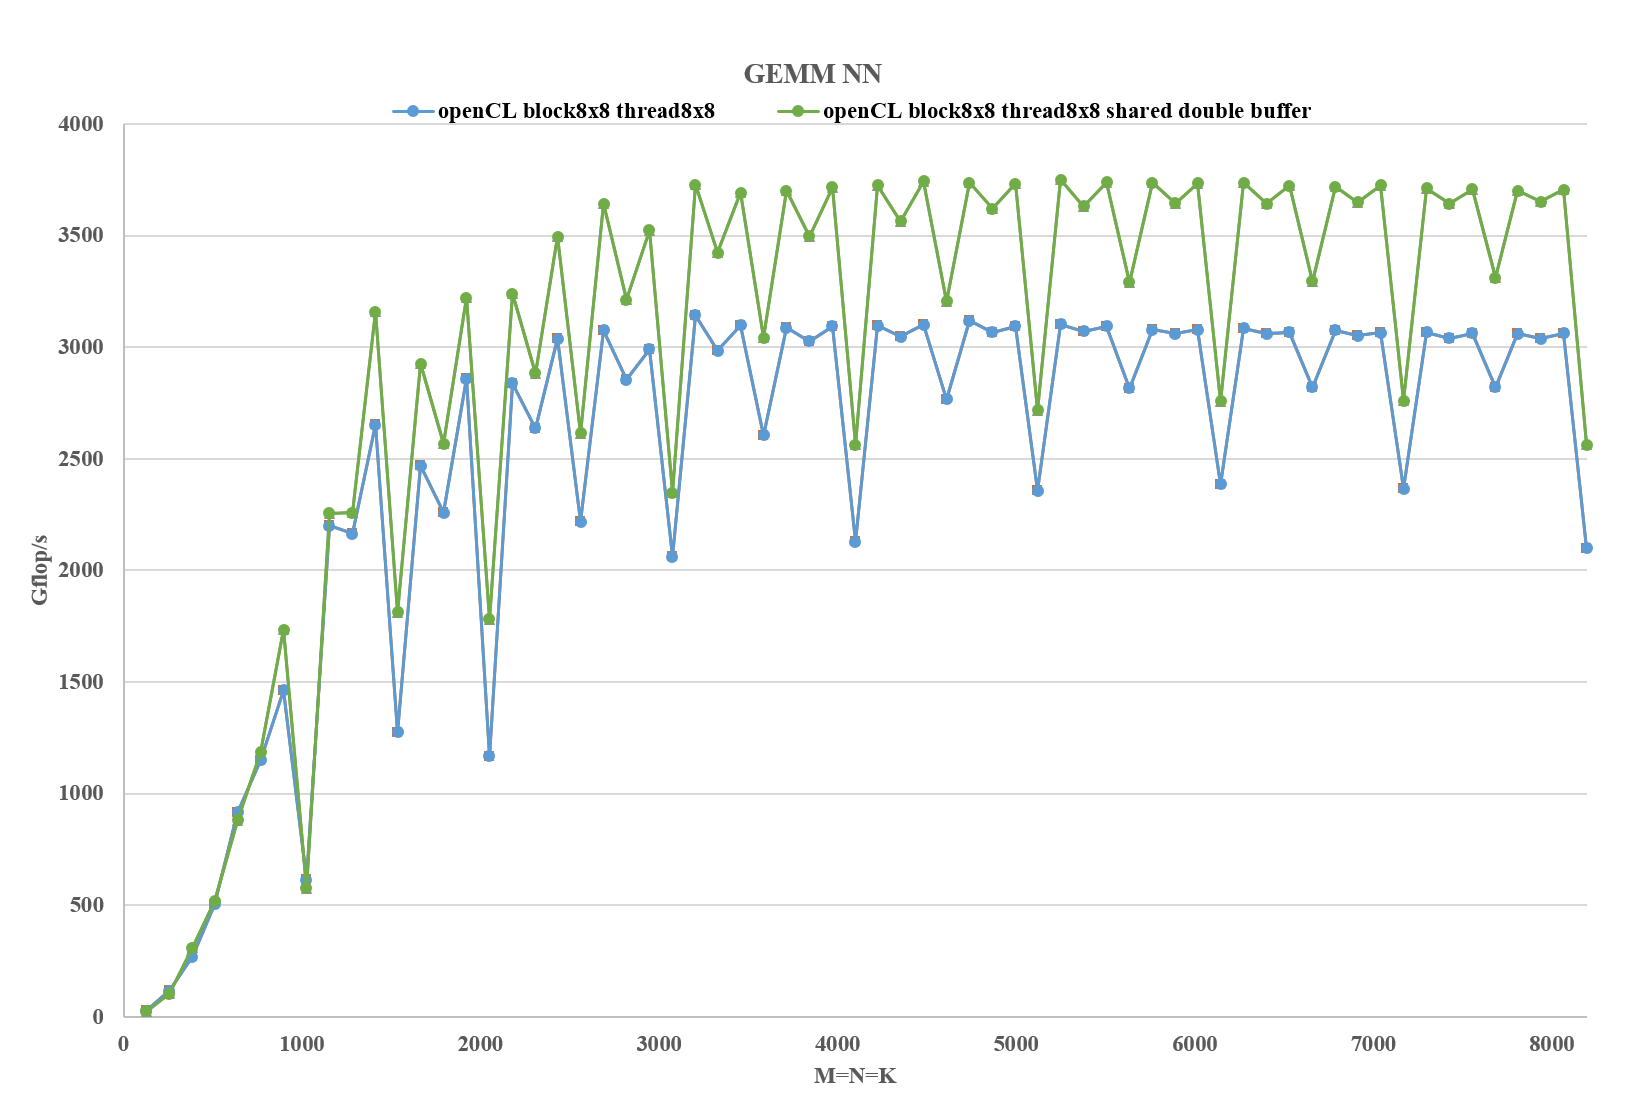
\includegraphics[width=0.80\textwidth]{gemm_shared_double_buffer_replot}
	\bicaption{shared memory双缓冲带来的性能提升}{Shared memory double buffering brings performance improvements}
	\label{fig:gemm_shared_double_buffer_replot}
\end{figure}

\begin{algorithm}[htbp]
	\small
	\caption{GEMM algorithm with shared memory double buffer variant1}\label{alg:gemm_sharedmem_v1}
	\begin{algorithmic}[1]
		%\Procedure{Euclid}{$a,b$}\Comment{The g.c.d. of a and b}
		\State $A, B, C$\Comment{matrix A, B, C}
		\State $regA[task\_size],regB[task\_size],regC[task\_size]$\Comment{Allocate register for compute}
		\State $tileA[tile\_length*NUM\_UNROLL],tileB[tile\_length*NUM\_UNROLL]$\Comment{Shared memory double buffer}
		\State $tileA'[tile\_length*NUM\_UNROLL],tileB'[tile\_length*NUM\_UNROLL]$
		\State $loadA[tile\_length*NUM\_UNROLL/threadblock]$\Comment{Register for global memory load}
		\State $loadB[tile\_length*NUM\_UNROLL/threadblock]$
		\State $regC \gets 0$
		\State $loadA \gets A, loadB \gets B $\Comment{Pre load tile of A, B from global to register}
		\State barrier CLK\_GLOBAL\_MEM\_FENCE
		\For   {$i = 0$; $i < K/NUM\_UNROLL$; $++i$}
			\If    {$i \% 2 == 0$}
				\State $tileA \gets loadA, tileB \gets loadB$
				\State barrier CLK\_LOCAL\_MEM\_FENCE
				\State $loadA \gets A, loadB \gets B $\Comment{Load the next tile of A, B from global to register}
				\State barrier CLK\_GLOBAL\_MEM\_FENCE
					\For   {$k = 0$; $k<NUM\_UNROLL$;$++k$}\Comment{Loop Unroll}
						\State $regA \gets tileA, regB \gets tileB$
						\State $regC \gets regA \cdot regB + regC$
					\EndFor
			\Else  
				\State $tileA' \gets loadA, tileB' \gets loadB$
				\State barrier CLK\_LOCAL\_MEM\_FENCE
				\State $loadA \gets A, loadB \gets B $\Comment{Load the next tile of A, B from global to register}
				\State barrier CLK\_GLOBAL\_MEM\_FENCE
					\For   {$k = 0$; $k<NUM\_UNROLL$;$++k$}\Comment{Loop Unroll}
						\State $regA \gets tileA', regB \gets tileB'$
						\State $regC \gets regA \cdot regB + regC$
					\EndFor
			\EndIf
		\EndFor\label{gemmendfor}
		\State $C \gets regC$\Comment{Store C from registers to global memory}
		%\EndProcedure
	\end{algorithmic}
\end{algorithm}
两种shared memory双缓冲实现方式的的比较,第一种算法\ref{alg:gemm_sharedmem_v1}实现中,barrier CLK\_GLOBAL\_MEM\_FENCE语句放在全局内存读语句之后;第二种算法\ref{alg:gemm_sharedmem_v2}实现中,barrier CLK\_GLOBAL\_MEM\_FENCE语句放在寄存器写入数据到shared memory之前。从直观理解上第二种算法\ref{alg:gemm_sharedmem_v2}的性能应该优于第二种,因为第二种实现中将给全局内存到寄存器的数据读操作的延迟留出了更多的等待时间。但在AMD ROCm平台上实测的结果是第一种实现要好于第二种(图\ref{fig:gemm_shared_double_buffer_v2_replot}),第三种算法\ref{alg:gemm_sharedmem_v3}的整体性能要好于前两种算法,这里没有了if-else分支判断,产生了微弱的性能优势。从这里可以看出,编程人员有时对GPU编译器的行为无法做出预测,影响了更为细致的调优工作的开展。
\begin{figure}[htbp]
	\centering
	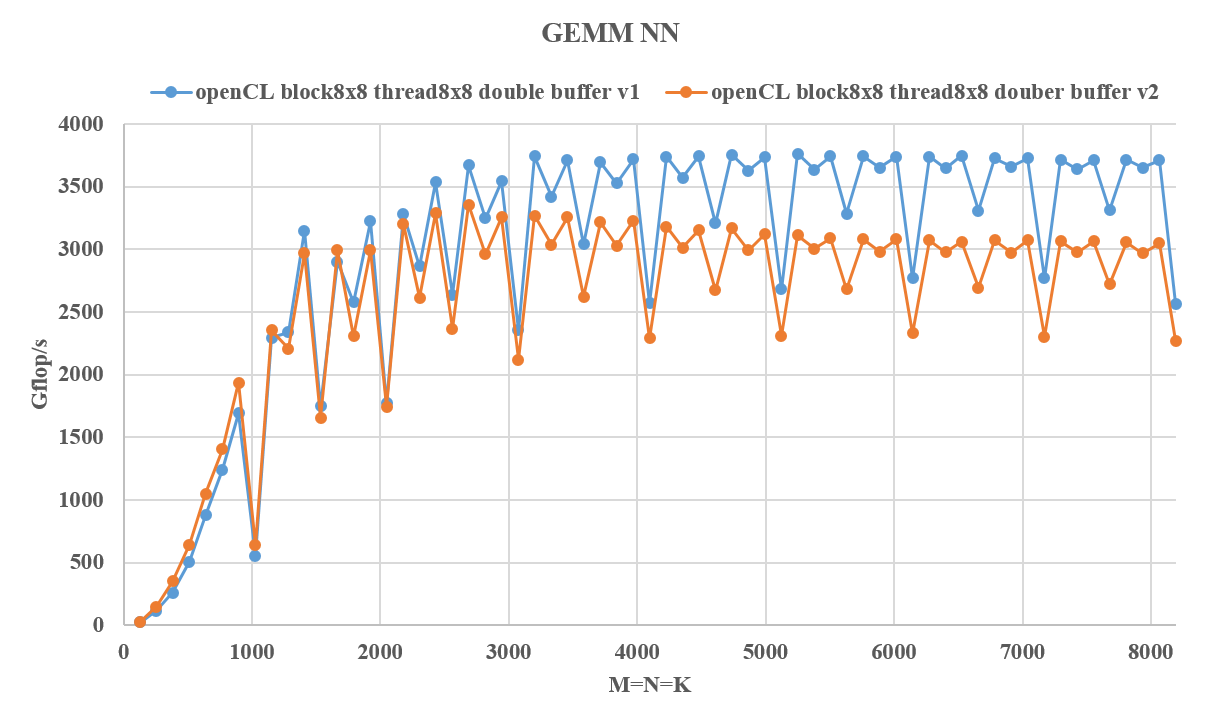
\includegraphics[width=0.80\textwidth]{gemm_shared_double_buffer_v2_replot}
	\bicaption{两种shared memory双缓冲实现的性能比较}{Performance comparison of two shared memory double buffering implementations}
	\label{fig:gemm_shared_double_buffer_v2_replot}
\end{figure}

\begin{algorithm}[htbp]
	\small
	\caption{GEMM algorithm with shared memory double buffer variant2}\label{alg:gemm_sharedmem_v2}
	\begin{algorithmic}[1]
		%\Procedure{Euclid}{$a,b$}\Comment{The g.c.d. of a and b}
		\State $A, B, C$\Comment{matrix A, B, C}
		\State $regA[task\_size],regB[task\_size],regC[task\_size]$\Comment{Allocate register for compute}
		\State $tileA[tile\_length*NUM\_UNROLL],tileB[tile\_length*NUM\_UNROLL]$\Comment{Shared memory double buffer}
		\State $tileA'[tile\_length*NUM\_UNROLL],tileB'[tile\_length*NUM\_UNROLL]$
		\State $loadA[tile\_length*NUM\_UNROLL/threadblock]$\Comment{Register for global memory load}
		\State $loadB[tile\_length*NUM\_UNROLL/threadblock]$
		\State $regC \gets 0$
		\State $loadA \gets A, loadB \gets B $\Comment{Pre load tile of A, B from global to register}
		\For   {$i = 0$; $i < K/NUM\_UNROLL$; $++i$}
		\If    {$i \% 2 == 0$}
		\State barrier CLK\_GLOBAL\_MEM\_FENCE
		\State $tileA \gets loadA, tileB \gets loadB$
		\State barrier CLK\_LOCAL\_MEM\_FENCE
		\State $loadA \gets A, loadB \gets B $\Comment{Load the next tile of A, B from global to register}
		\For   {$k = 0$; $k<NUM\_UNROLL$;$++k$}\Comment{Loop Unroll}
		\State $regA \gets tileA, regB \gets tileB$
		\State $regC \gets regA \cdot regB + regC$
		\EndFor
		\Else
		\State barrier CLK\_GLOBAL\_MEM\_FENCE  
		\State $tileA' \gets loadA, tileB' \gets loadB$
		\State barrier CLK\_LOCAL\_MEM\_FENCE
		\State $loadA \gets A, loadB \gets B $\Comment{Load the next tile of A, B from global to register}
		\State barrier CLK\_GLOBAL\_MEM\_FENCE
		\For   {$k = 0$; $k<NUM\_UNROLL$;$++k$}\Comment{Loop Unroll}
		\State $regA \gets tileA', regB \gets tileB'$
		\State $regC \gets regA \cdot regB + regC$
		\EndFor
		\EndIf
		\EndFor\label{gemmendfor}
		\State $C \gets regC$\Comment{Store C from registers to global memory}
		%\EndProcedure
	\end{algorithmic}
\end{algorithm}

\subsection{寄存器双缓冲}
如图\ref{fig:reg_double_buffer_replot}所示,可以在用寄存器A1,B1计算的同时,从局部共享内存取下一次要计算的数据到寄存器A0,B0。由于数据的预取,在进入循环前,已经将第一次要计算的数据读到了寄存器A0[0:7],B0[0:7]中。

每个线程使用A1,B1寄存器中的数据,做本次的8x8乘加操作;在线程做本次乘加操作的同时,从局部共享内存预取下一次的数据到寄存器A0,B0。通过寄存器双缓冲,可以用计算掩盖从局部共享内存读的延迟。沿着K方向循环展开8次,分成0,2,4,6 和 1,3,5,7。一半奇数,一半偶数。偶数次时,每个线程从shared memory预取8个a到寄存器A1[0:7],8个b到寄存器B1[0:7], 即预取下一次(奇数时)计算需要的8个a和8个b。奇数次时,每个线程从shared memory预取8个a到寄存器A0[0:7],8个b到寄存器B0[0:7], 即预取下一次(偶数时)计算需要的8个a和8个b。偶数次循环计算A0[0:7]*B0[0:7],奇数次循环计算 A1[0:7]*B1[0:7]。对每个线程来说,需要计算8x8个输出,共需要做64次乘加操作。从共享内存读,一次读4个连续元素,读8个a和8个b,需要4个共享内存读指令。这样就可以用寄存器的计算,来掩盖共享内存读的延迟。

\begin{figure}[htbp]
	\centering
	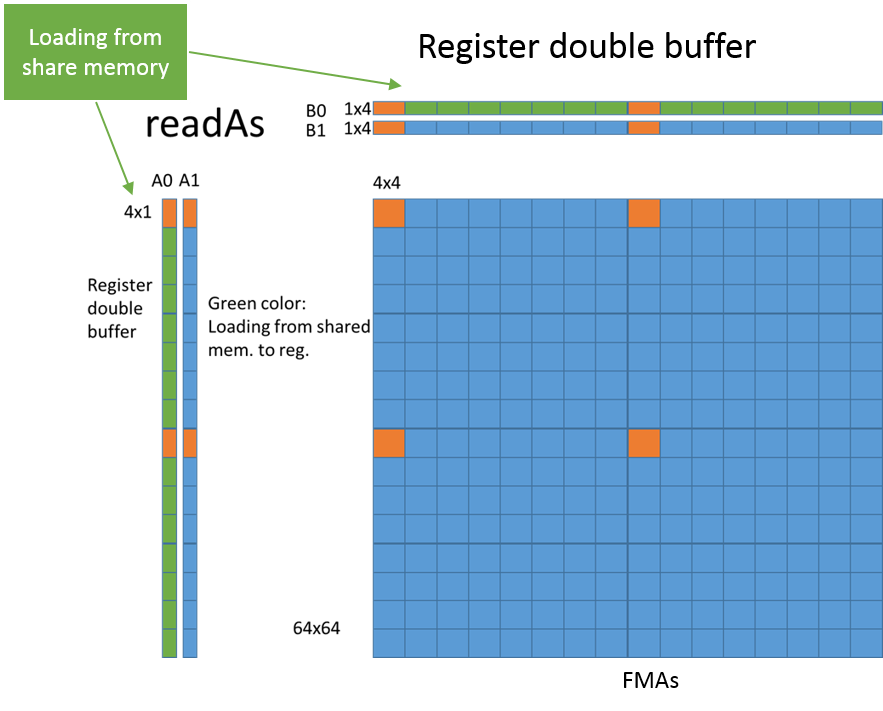
\includegraphics[width=0.50\textwidth]{reg_double_buffer_replot}
	\bicaption{寄存器双缓冲}{Register double buffer}
	\label{fig:reg_double_buffer_replot}
\end{figure}

\begin{algorithm}[htbp]
	\small
	\caption{GEMM algorithm with shared memory double buffer variant3}\label{alg:gemm_sharedmem_v3}
	\begin{algorithmic}[1]
		%\Procedure{Euclid}{$a,b$}\Comment{The g.c.d. of a and b}
		\State $A, B, C$\Comment{matrix A, B, C}
		\State $regA[task\_size],regB[task\_size],regC[task\_size]$\Comment{Allocate register for compute}
		\State $tileA[tile\_length*NUM\_UNROLL],tileB[tile\_length*NUM\_UNROLL]$\Comment{Shared memory double buffer}
		\State $tileA'[tile\_length*NUM\_UNROLL],tileB'[tile\_length*NUM\_UNROLL]$
		\State $loadA[tile\_length*NUM\_UNROLL/threadblock]$\Comment{Register for global memory load}
		\State $loadB[tile\_length*NUM\_UNROLL/threadblock]$
		\State $regC \gets 0$
		\State $loadA \gets A, loadB \gets B $\Comment{Pre load tile of A, B from global to register}
			\For   {$i = 0$; $i < K/NUM\_UNROLL$; $++i$}
				\State barrier CLK\_GLOBAL\_MEM\_FENCE
				\State $tileA \gets loadA, tileB \gets loadB$
				\State barrier CLK\_LOCAL\_MEM\_FENCE
				\State $loadA \gets A, loadB \gets B $\Comment{Load the next tile of A, B from global to register}
					\For   {$k = 0$; $k<NUM\_UNROLL$;$++k$}\Comment{Loop Unroll}
						\State $regA \gets tileA, regB \gets tileB$
						\State $regC \gets regA \cdot regB + regC$
					\EndFor
				\State $tileA \leftrightarrow tileA', tileB \leftrightarrow tileB'$\Comment{Swap double buffer}
			\EndFor\label{gemmendfor}
		\State $C \gets regC$\Comment{Store C from registers to global memory}
		%\EndProcedure
	\end{algorithmic}
\end{algorithm}

\subsection{线程负载均衡}
对每个线程来说,使用4个4x4,来代替8x8的计算方式,来使得一个block中的线程可以负载均衡(如图\ref{fig:load_balance_replot})。在进行shared memory bank冲突消除时,同时做到了线程的负载均衡。将一个threadblock的计算任务均等的划分成4份。所有线程都分别计算4份中的每一个中相应的元素。例如,0号线程分别计算4个分块的左上角的4x4的输出。通过这种方式,可以提高一个block的计算效率。
\begin{figure}[htbp]
	\centering
	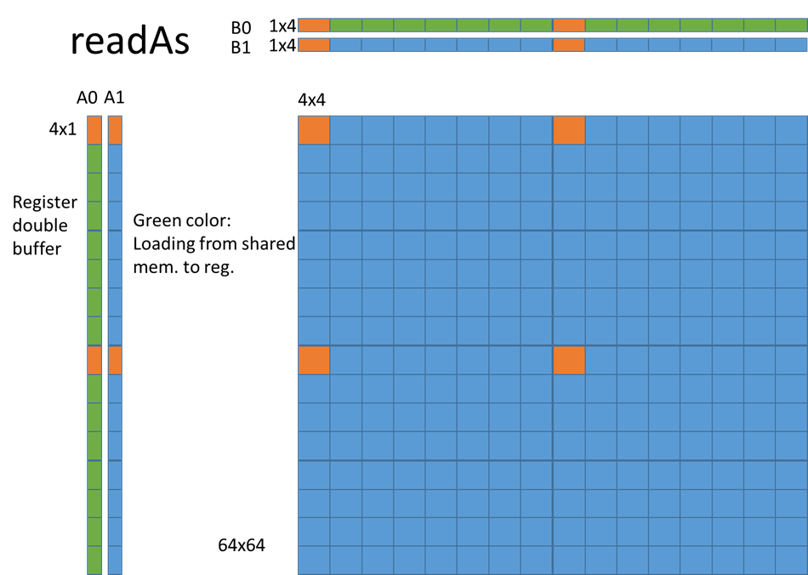
\includegraphics[width=0.50\textwidth]{load_balance_replot}
	\bicaption{线程负载均衡}{Thread load balance}
	\label{fig:load_balance_replot}
\end{figure}


\subsection{消除shared memory bank冲突}
AMD GPU shared memory有32个bank。当不同的线程访问不同的bank时,线程可以同时读;当不同的线程访问同一个bank的同一个位置时,可以进行广播;当不同的线程访问同一个bank的不同位置时,会产生bank冲突,需要多个时钟周期来完成。所以,bank冲突会减小访存带宽,对性能影响很大。

在前面的6.3.1小结中,分析了外积法的原始实现中,有4-way shared memory bank冲突。通过观察可以发现,产生shared memory bank冲突的原因是在一个threadblock中,所有线程对shared memory的访问跨越了2个bank,导致不同的线程访问同一个的bank的不同entry这种情况发生。接下来,将展示如何通过分配线程的计算任务来消除shared memory bank冲突。消除shared memory bank冲突的方法是安排一个thread block中的所有线程对shared memory的一次访问限制在一个bank中。图\ref{fig:gemm_no_bank_conflict_replot}展示了通过消除shared memory bank冲突所带来的性能提升。从图\ref{fig:gemm_no_bank_conflict_replot}看出,通过消除bank冲突可以带来微弱的性能提升,这里的一个原因是这里的shared memory bank冲突消除是在原始的外积法矩阵乘的基础上实现的。此时矩阵乘瓶颈还在全局访存。没有用到shared memory双缓冲,因此提升的性能不多。

\begin{figure}[htbp]
	\centering
	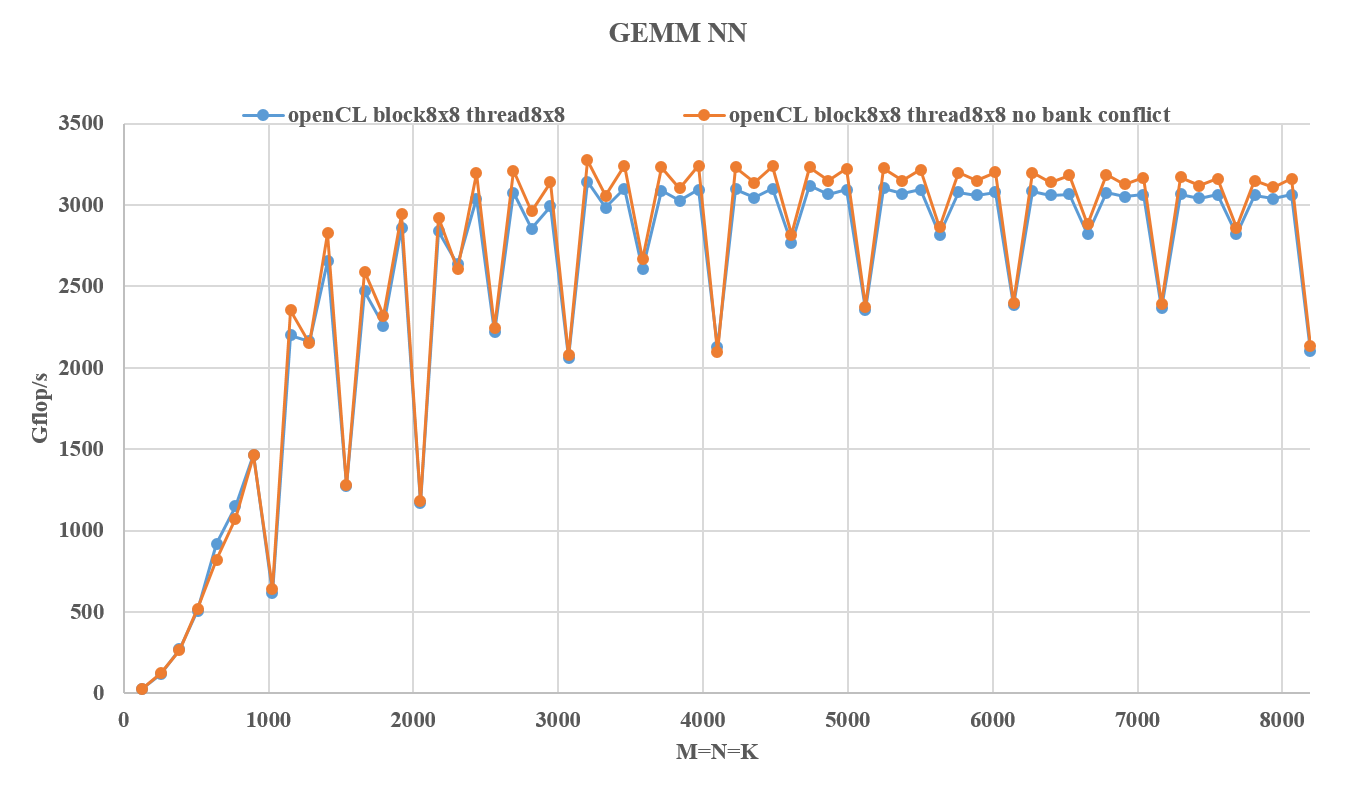
\includegraphics[width=0.80\textwidth]{gemm_no_bank_conflict_replot}
	\bicaption{shared memory bank冲突消除带来的性能提升}{Performance improvements with shared memory bank conflict elimination}
	\label{fig:gemm_no_bank_conflict_replot}
\end{figure}


图\ref{fig:gemm_shared_db_no_bank_conflict_replot}展示了在外积法原始实现版本中分别加入shared memory双缓冲和bank冲突消除优化手法所带来的性能提升。
\begin{figure}[htbp]
	\centering
	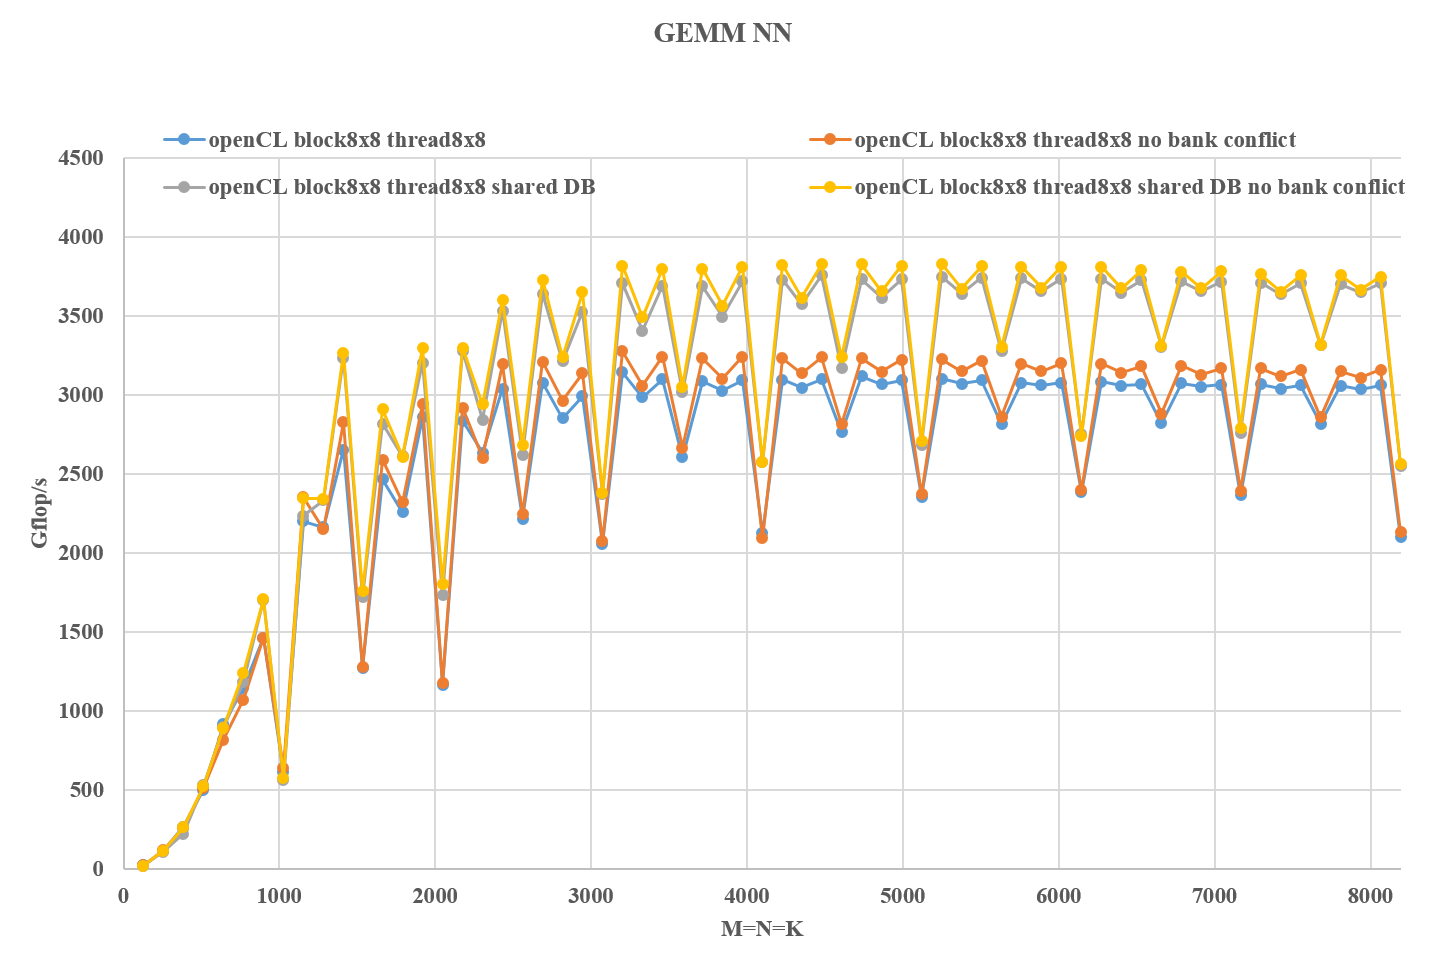
\includegraphics[width=0.80\textwidth]{gemm_shared_db_no_bank_conflict_replot}
	\bicaption{shared memory 双缓冲,无bank冲突的性能表现}{GEMM performance with shared memory DB and bank conflict elimination}
	\label{fig:gemm_shared_db_no_bank_conflict_replot}
\end{figure}
图\ref{fig:bank_conflict_replot}中小方格中的数字表示一个block中的64个线程,将64个线程看成一个2维的线程数组tid.x 取值为0$\sim$7, tid.y取值为0$\sim$7。小方格中的数字对(tid.x,tid.y)对应的线程号为tid = tid.y * 8 + tid.x。可以看到,图\ref{fig:bank_conflict_replot}中同一行的线程读4个连续的bank,没有bank冲突;不同线程读相同的位置,会在同一行进行广播;图中同一列的线程读4个连续的bank没有bank冲突会在同一列进行广播。因此通过设计这种共享内存读的方式可以完全消除bank冲突。
\begin{figure}[htbp]
	\centering
	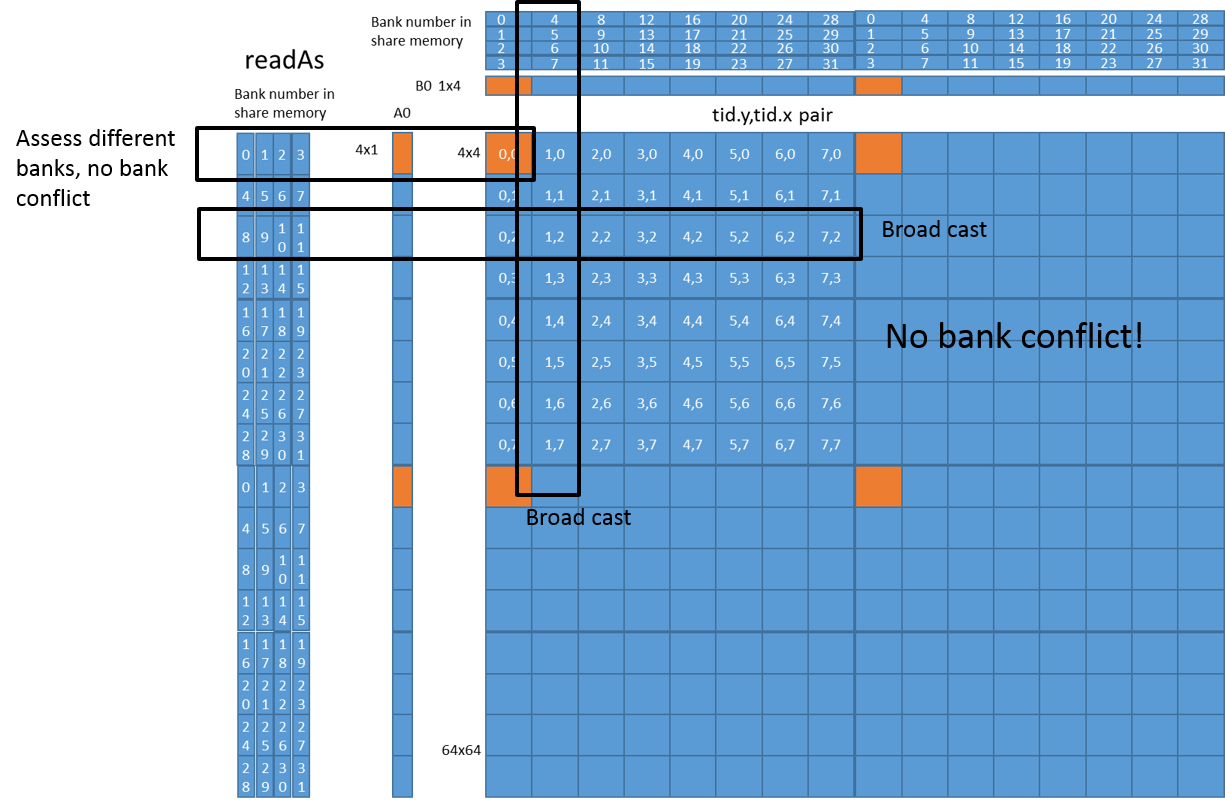
\includegraphics[width=0.70\textwidth]{bank_conflict_replot}
	\bicaption{shared memory bank冲突消除}{Shared memory bank conflict elimination}
	\label{fig:bank_conflict_replot}
\end{figure}


\subsection{指令重排}
通常编程人员尝试将不同类型的指令交错放置来使得一个CU上不同的功能部件可以均衡的利用起来,进而获得更高的指令通量。本文采用下面的指令重排方法。将全局内存数据预取指令和v\_mac,DS\_READ指令交错放置来获得更高的性能。图\ref{fig:none_f_mac_inst}展示了矩阵乘主循环中非v\_mac指令的位置。
\begin{figure}[htbp]
	\centering
	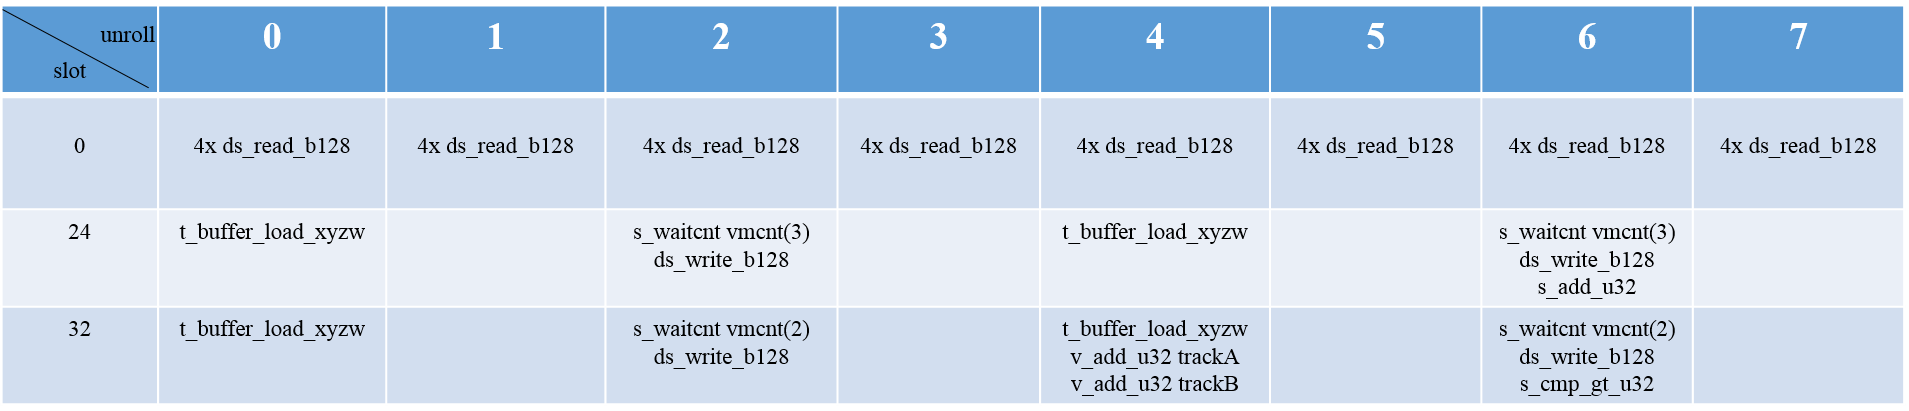
\includegraphics[width=1.0\textwidth]{none_f_mac_inst}
	\bicaption{非v\_mac指令的位置}{None v\_mac inst slot}
	\label{fig:none_f_mac_inst}
\end{figure}

%	
%\begin{table}[!htbp]
%	\bicaption{非v\_mac指令的位置}{Instruction position of the none v\_mac}
%	\label{tab:thread_data_move}
%	%\centering
%	\begin{center}
%		 \resizebox{\textwidth}{18mm}{ 
%		\begin{tabular}{|l|l|l|l|l|l|l|l|l|}
%			\hline
%			\diagbox {slot}{unroll} & $0$ & $1$ & $2$ & $3$ & $4$ & $5$ & $6$ & $7$\\ %添加斜线表头
%			\hline
%			$0$ & 4x ds\_read\_b128 & 4x ds\_read\_b128 & 4x ds\_read\_b128 & 4x ds\_read\_b128 & 4x ds\_read\_b128 & 4x ds\_read\_b128 & 4x ds\_read\_b128 & 4x ds\_read\_b128 \\
%			\hline
%			\multirow{3}*{$24$} & t\_buffer\_load\_xyzw  &  & s\_waitcnt vmcnt(3)& & t\_buffer\_load\_xyzw & & s\_waitcnt vmcnt(3) & \\
%			~                   &                        &  & ds\_write\_b128    & &                       & & ds\_write\_b128     & \\
%			~                   &                        &  &                    & &                       & & s\_add\_u32         & \\
%			\hline
%			%$24$ & t\_buffer\_load\_xyzw  &  & s\_waitcnt vmcnt(2)  ds\_write\_b128 & & t\_buffer\_load\_xyzw v\_add\_u32 trackA v\_add\_u32 trackB & & s\_waitcnt vmcnt(3) ds\_write\_b128 s\_cmp\_gt\_u32 & %\\
%			\hline
%		\end{tabular}}
%	\end{center}
%\end{table}
%	
%%\end{document}


\subsubsection{指令重排的几个原则}
(1) 从shared memory中预取数据到寄存器的指令:尽可能地早放置。

ds\_read\_b128指令用于从shared memory中预取数据到寄存器。循环展开8次,每次计算8x8个输出。总共8x8x8 = 512条v\_mac指令。一条ds\_read\_b128指令可以从shared memory中取4个浮点元素。计算8x8的输出需要8个A中对应元素和8个B中对应元素,因此需要(8+8)/4 = 4 条ds\_read\_b128指令。在计算本次8x8个v\_mac时,要预取下一个8x8个v\_mac所需的指令。为了给ds\_read\_b128指令从发射到结果返回留出足够多的时间,放置ds\_read\_b128指令的原则是尽可能地早发射ds\_read\_b128指令,所以在每次8x8个v\_mac最开始的位置之前插入4条ds\_read\_b128指令。

(2) 从全局内存读取数据到寄存器:尽可能地早放置。

t\_buffer\_load\_xyzw指令用于从全局内存预取数据到寄存器。一个block有64个线程,每个线程计算8x8个输出,总共可以计算64x64个输出。t\_buffer\_load\_xyzw指令一次可以从全局内存读取4个元素,计算64x64的输出,循环展开8次,需要8x64个A中对应元素和8x64个B中对应元素。因此每个线程需要(8x64+8x64)/(4x64) = 4条t\_buffer\_load\_xyzw指令。(3) 从寄存器写入数据到shared memory:和全局内存读指令间隔足够远。

为了数据重用,把从全局内存读到寄存的数据写入shared memory。使用ds\_read\_b128指令将数据从存寄存器写入shared memory。ds\_read\_b128指令要等对应的t\_buffer\_load\_xyzw指令结果返回,所以ds\_read\_b128指令和t\_buffer\_load\_xyzw要间隔得足够远。

从图\ref{fig:none_f_mac_inst}可以观察出在每个8x8的循环的起始位置插入4条ds\_read\_b128指令,这4条指令是为下一个8x8循环进行预取。在第0次展开的24和32的位置插入两条全局内存读指令t\_buffer\_load\_xyzw,这两条指令也是在进行数据预取。为了让全局内存读指令和共享内存写指令间隔的尽可能地远,在第6次展开的24和32位置插入共享内存写指令ds\_write\_b128。其中最为巧妙的是利用s\_waitcnt vmcnt()指令来精确地等待某一条全局内存读指令的完成。第6次展开的24位置s\_waitcnt vmcnt(3)指令表示3条全局访存指令还未完成,即按顺序发射了4条访存指令,其中第1条访存指令结果已经返回,剩下3条指令结果还未返回,这样就是在等待第1条指令结果返回然后继续执行,否则就等待。其他指令的位置可类似分析。同时相比于OpenCL,手工编写汇编可以去除冗余指令,在OpenCL中只能使用barrier指令来进行等待,手工编写汇编可以去除barrier指令使用更为准确的s\_waitcnt指令进行等待。


\section{矩阵乘性能测试}
通过实际测试(如图\ref{fig:hgemm_perf}),矩阵乘性能峰值可达$\sim$95\%。图\ref{fig:gemm_tuning_comp}展示了分别采用循环展开,shared memory双缓冲,bank冲突消除,寄存器双缓冲和指令重排所带来的一步步性能提升。对比了AMD官方库rocBLAS和Tensile,相比roclBLAS,最高有$\sim$20\%的性能提升,对比自动调优库Tensile生成的汇编矩阵乘有略微的性能优势,最多有3\%$\sim$5\%的性能提升。
\begin{figure}[htbp]
	\centering
	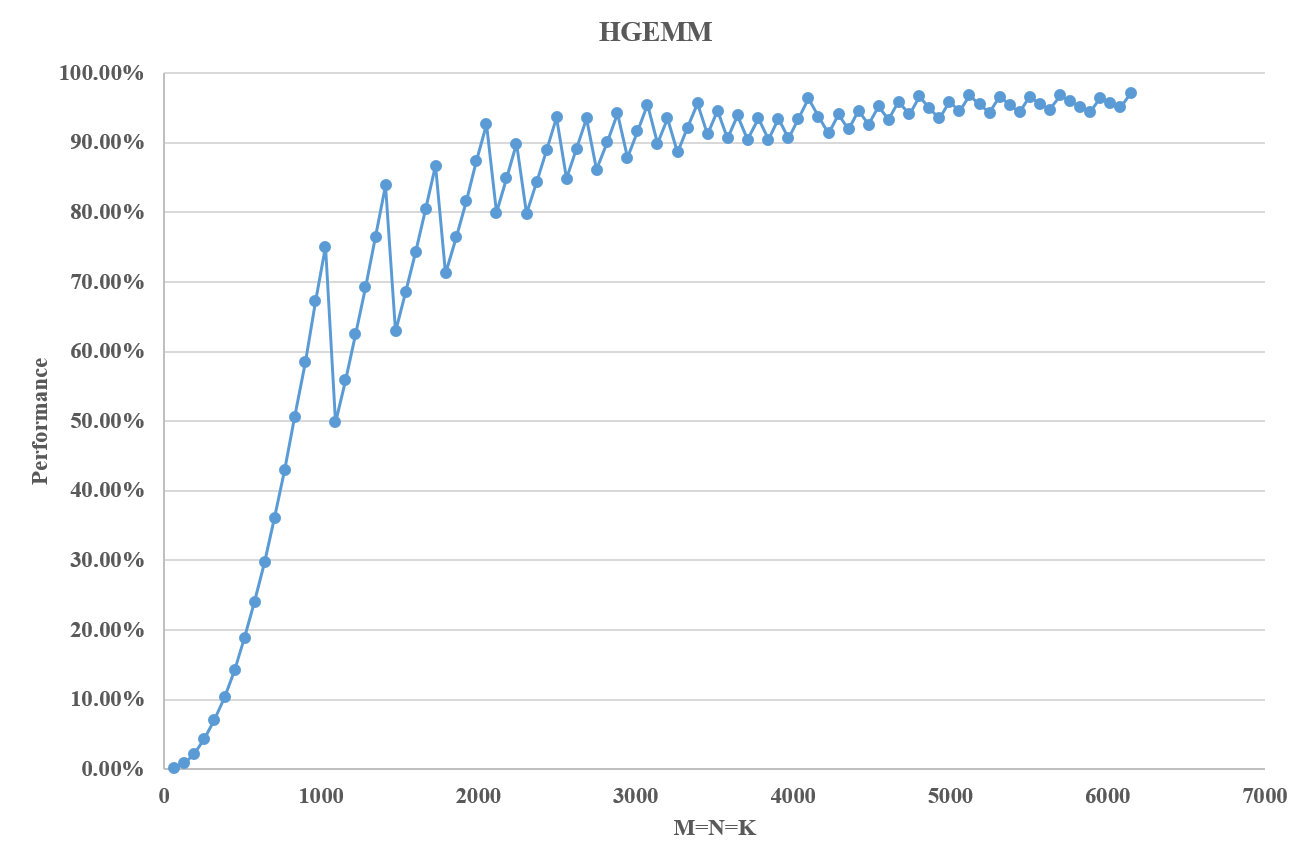
\includegraphics[width=0.80\textwidth]{hgemm_perf}
	\bicaption{汇编调优的矩阵乘性能展示}{GEMM performance}
	\label{fig:hgemm_perf}
\end{figure}
\begin{figure}[htbp]
	\centering
	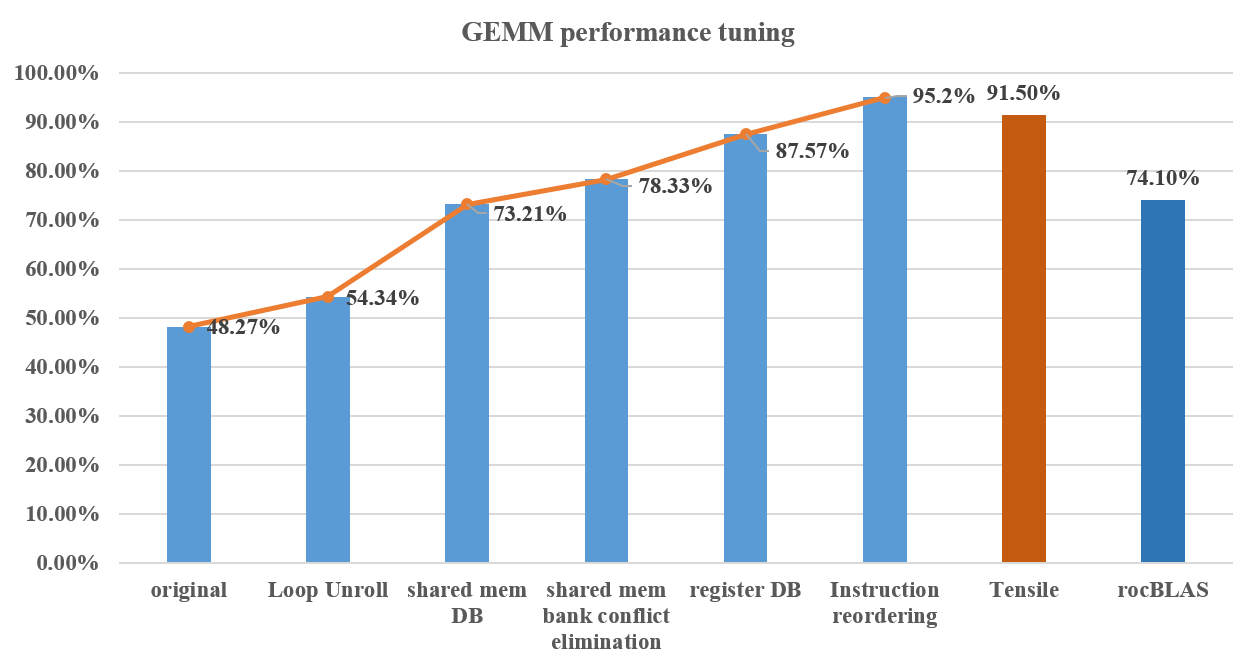
\includegraphics[width=0.80\textwidth]{gemm_tuning_comp}
	\bicaption{矩阵乘性能变化趋势}{GEMM performance tuning}
	\label{fig:gemm_tuning_comp}
\end{figure}
这里需要说明的是在本次测试中使用的矩阵规模都是正方形,即M=N=K的情况,并且都是64的整数倍,并且对非64整数倍的矩阵尺寸没有进行边界处理。其中循环展开,shared memory双缓冲和寄存器双缓冲带来了大部分的性能能提升,这得益于利用shared memory和寄存器隐藏了全局内存读延迟。

指令细粒度重排只有用汇编才可实现,OpenCL可以使用的同步指令只有barrier CLK\_GLOBAL\_MEM\_FENCE和barrier CLK\_LOCAL\_MEM\_FENCE这两种;而在汇编语言中,通过使用s\_waitcnt vmcnt()可以具体等待某一条访存指令的完成,同时,也没有OpenCL编译器所带来的无法预测的行为。通过利用前面讲到的指令重排的几个原则,进一步掩盖访存延迟,获得计算性能的提升。


\section{矩阵乘性能分析}
\subsection{矩阵乘潜在性能峰值}
在寄存器分块大小为8x8,block线程数为64的情况下。v\_mac峰值性能为512/(512+24+2) = 512/538 = 95.17\%。这里在计算上认为32条ds\_read\_b128有只有8条指令双发射。实际处理器的执行行为需要通过测试可以得知。
\begin{table}[htbp]
	\bicaption{矩阵乘主循环指令构成}{GEMM main loop instructions}
	\label{tab:fijiFFMA}
	\begin{center}
		\begin{tabular}{ | l | p{4cm} |}
			\hline
			Operation & Count \\ \hline
			v\_mac & 512  \\ \hline
			ds\_read\_b128 & total 32, 8 dual issue \\ \hline
			ds\_write\_b128 & 4 dual issue \\ \hline
			tbuffer\_load\_xyzw & 4 dual issue \\ \hline
			v\_add\_u32 & 2 \\ \hline
			s\_waitcnt vmcnt() & 4 dual issue \\ \hline
			s\_add\_u32 & 1 dual issue \\ \hline
			s\_cmp\_gt\_u32 & 1 dual issue \\ \hline
			s\_cbranch\_scc0 & 1 daul issue \\
			\hline
		\end{tabular}
	\end{center}	
\end{table}

如果在执行时,将每4条ds\_read\_b128指令合并,则32条ds\_read\_b128全部都双发射。此时的v\_mac峰值性能为512/(512+2) = 99.61\%(如表\ref{tab:fijiFFMA})。

\subsection{Roofline模型}
Roofline\citepns{williams2009roofline}模型是Williams和Patterson等人在2008年提出的一个可视化应用程序性能分析模型,用于分析多核计算机系统上的浮点计算程序性能。该模型为并行软件和多核计算机体系结构的设计提供了有用的指导。Roofline模型从计算量和访存量这两个方面来描述浮点计算程序和多核计算机体系结构的性能。当浮点部件未充分使用时,随着内存带宽的提升浮点计算性能跟着提升,此时的程序性能瓶颈为内存带宽受限;当浮点部件被完全使用时,随着内存带宽的提升浮点计算性能不再变化,此时的程序性能瓶颈为计算受限。
\begin{equation}
\label{eq:global_arith_intensity}
gmemAI = \frac{2 \times b_m \times b_m \times b_k}{4\times (b_m \times b_k + b_n\times b_k)} = \frac{Gflops}{bandwidth}
\end{equation}

\begin{figure}[htbp]
	\centering
	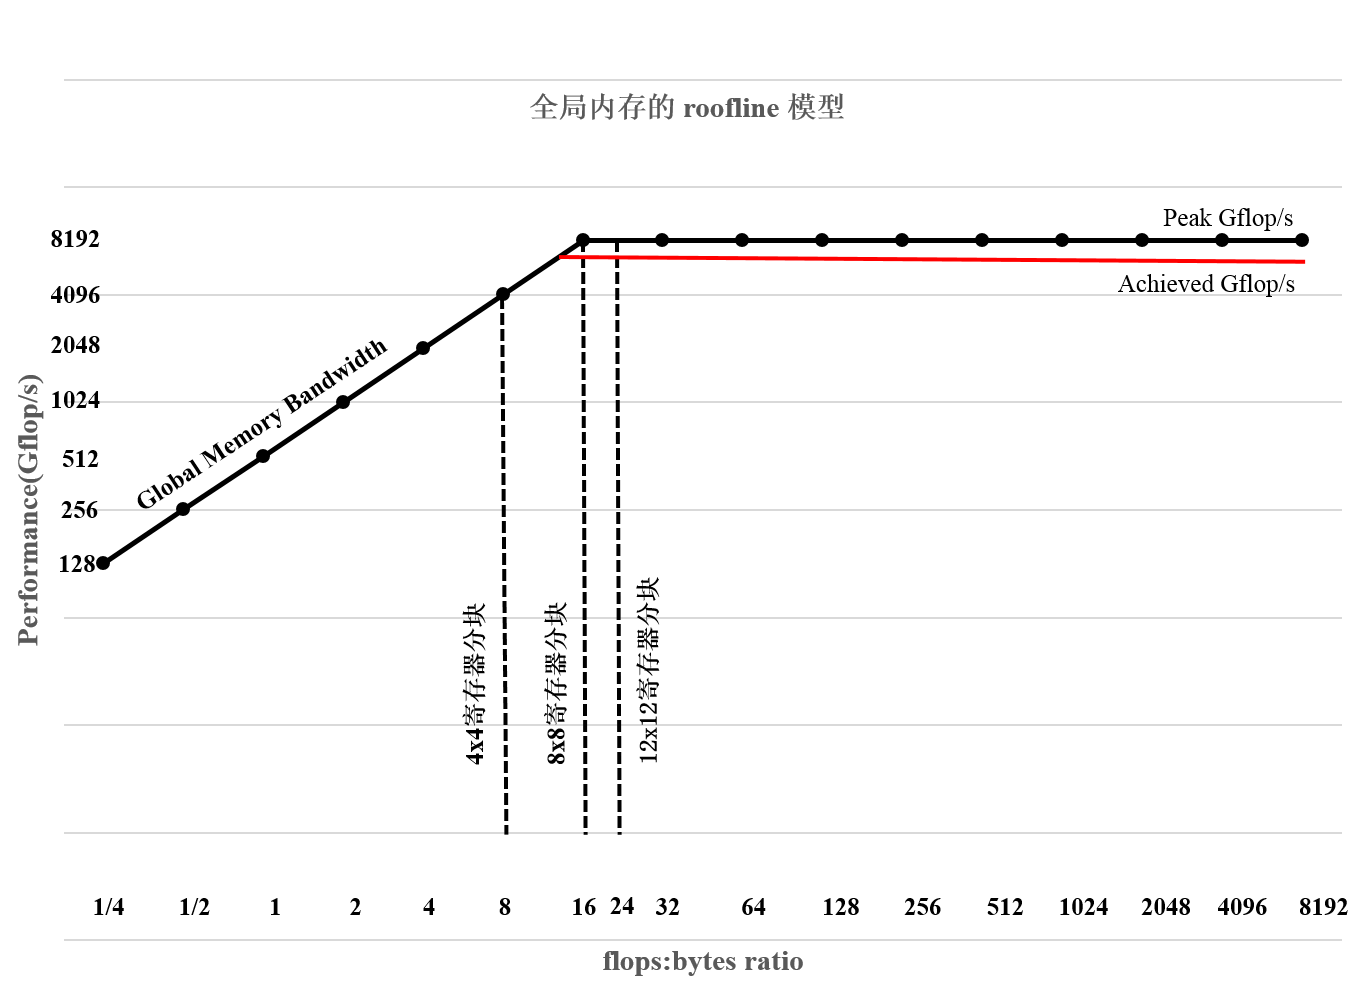
\includegraphics[width=1.0\textwidth]{roofline_global}
	\bicaption{全局内存的roofline模型}{Global memory roofline model}
	\label{fig:roofline_global}
\end{figure}

图\ref{fig:roofline_global}展示了AMD Fiji GPU的全局内存Roofline模型,黑色实线代表机器理论峰值,横坐标为计算和全局内存访存比例,纵坐标为机器理论浮点峰值。在矩阵乘的主循环中,每个线程块计算量为$2\times b_m \times b_n \times b_k$次浮点操作,访存量为$4\times (b_m \times b_k + b_n\times b_k)$个字节,因此每个线程块的计算和全局内存访存比例(Global memory arithmetic intensity)可由公式\ref{eq:global_arith_intensity}计算得出。

在我们实现的矩阵乘算法中,$b_m = b_n = 64$,$b_k = 8$。AMD Fiji GPU的最高浮点性能为8192 Gflop/s,对全局内存带宽的最低要求是512 GB/s。Fiji GPU可以提供的全局访存带宽为$Global_{bandwidth} = 2 \times f_{mem} \times W = 2 \times 500MHz \times 4096bit = 512GB/s$,可以满足矩阵乘算法对全局访存带宽的要求。可以看到$4\times 4$寄存器分块算法的计算访存比为8,其对应的浮点性能峰值为4096 Gflop/s,此时矩阵乘的性能严重受到全局内存访存带宽的限制;$8\times 8$寄存器分块算法正好处在Roofline模型的拐点处,矩阵乘不受全局内存访存带宽的限制。寄存器分块越大,计算和全局内存访存比例越大,越接近机器理论峰值。


\section{本章小结}
本章首先介绍了本次实验所使用的计算环境,然后分析了寄存器分块的大小和读数据指令的位宽对浮点通量的影响,接下来详细描述了矩阵乘调优的过程。分别展示了循环展开、shared memory双缓冲、bank冲突消除、寄存器双缓冲和指令重排这些优化方法所带来的一步步性能提升,并和AMD官方数学库rocBLAS和Tensile的矩阵乘性能进行了对比。其中循环展开,shared memory双缓冲和寄存器双缓冲带来了大部分的性能能提升,这得益于利用shared memory和寄存器隐藏了全局内存读延迟。指令细粒度重排只有用汇编编写才能实现,因为在OpenCL层面,可以使用的同步指令只有barrier CLK\_GLOBAL\_MEM\_FENCE和barrier CLK\_LOCAL\_MEM\_FENCE这两种;而在汇编语言中,通过使用s\_waitcnt vmcnt()可以具体等待某一条访存指令的完成,同时,也没有OpenCL编译器所带来的无法预测的行为。通过利用前面讲到的指令重排的几个原则,进一步掩盖访存延迟,获得计算性能的提升。最后通过统计主循环中每种指令的个数和单双发射的情况,进行了矩阵乘性能上界分析。

